\section{Reinforcement Learning}
In this section I will introduce the Reinforcement Learning (RL)
paradigm. Then, its integration with deep learning is explored, and
subsequent improvements in the algorithm are also elaborated upon.
The end result, the Rainbow DQN agent, is integrated as part of the \textbf{System Design and Specification}.
\subsection{Markov Decision Processes}
A finite markov chain is a process that consists of a set of states
$\mathbf{S^n} \coloneqq \{S_1, S_2, \hdots, S_n\}$ and a transition
function $F(\mathbf{S})$ that takes the state at the current
timestep $t$ and outputs a new state at timestep $t+1$.
\begin{equation}
    F(S_t) \mapsto S_{t+1} \;\;\;\; \forall S \in \mathbf{S}, \forall t\in \mathbf{T}
\end{equation}
For a given process, the states are linked by a transition probability
$P(S_{t+1}, S_t)$. A process is markov only if the markov property holds:
\begin{equation}
    P(S_{t+1}, S_t) = P(S_{t+1} | S_t) \\
\end{equation}
The next state in a process that obeys the markov property is determined
solely by the value of the current state, and for any given sequence, the transition
probability between any two states remains the same. Thus, markov chains can begin
characterised by a transition matrix $\mathbf{P} \coloneqq |\mathbf{S}^n| \times |\mathbf{S}^n|$
where each row $j$ is a distribution $P(i, \cdot)$ such that:
\begin{equation}
    i \in \mathbf{S}^n, \sum_{j \in \mathbf{S}^n} P(i,j) = 1
\end{equation}\\
The product along the column space $j \in \mathbf{S}^n,{\displaystyle \prod_{i \in \mathbf{S}^n}} P(i,j)$ of the transition matrix reveals
the stationary probability of being in any particular state $P(S_j)$.
\begin{center}
    \begin{tikzpicture}[->,>=stealth',shorten >=1pt,auto,node distance=2.8cm,
        semithick,]
    \tikzstyle{every state}=[fill=white,draw=none,text=black,draw=black]
  
    \node[state] (A)                    {$S_1$};
    \node[state]         (B) [above right of=A] {$S_2$};
    \node[state]         (D) [below right of=A] {$S_3$};
    \node[state]         (C) [below right of=B] {$S_4$};
    \node[state]         (E) [below of=D]       {$S_5$};
    
    \path (A) edge              node {0.42} (B)
    edge              node {0.58} (C)
    (B) edge [loop above] node {0.6} (B)
    edge              node {0.4} (C)
    (C) edge              node {0.82} (D)
    edge [bend left]  node {0.18} (E)
    (D) edge [loop above] node {0.35} (D)
    edge              node {0.65} (A)
    (E) edge   node {0.2} (D)
    (E) edge [bend left]  node {0.8} (A);
    \end{tikzpicture}
    \captionof{figure}{Markov chain with state space and transition propabilities}
\end{center}
A Markov Decision Process (MDP) is a generalisation of this framework to sequential
decision making \cite{sutton2018reinforcement}. An MDP consists of an agent-environment
interface, where the \emph{Agent} is the learner and decision maker and the \emph{Environment}
consists of everything outside of the agent. The agent interacts with the environment
bny taking action $a \in \mathbf{A}$ in the current state $S_t$ and receives a reward $R_{t+1}$\footnote{Reward received at $t+1$ to indicate the fact that 
an action must be taken first to move to a new state in order to obtain a reward}, the outcome of the agents actions
transitions the environment from state $S_t$ to $S_{t+1}$.
The agent's long term reward is maximised by taking actions that move the agents into 
favourable states that yield higher rewards, the \textbf{expected} reward in any given state
is equal to the probability of entering state $S_{t+1}$ multiplied by the value of the reward $R_{t+1}$ in that state.
\begin{equation}
    {\displaystyle \E_{S \in \mathbf{S}^n}\biggl[R_{t+1} \; | \; S_t, A_t \biggl] = 
    P(R_{t+1}\; | \; S_t, A_t)\cdot R_{t+1}}
\end{equation}
The \emph{value} of a given state $\mathcal{V}(S)$ is the total expected reward for that state for any action taken in that state.
This is taken to be the \emph{long run} return of state $S$ if the process was repeated in the infinite limit under a stationary distribution of rewards\footnote{
    "Stationary" indicating that the probability of receiving a reward in any state does not change as the process evolves
}:
\begin{equation}
    { \displaystyle \mathcal{V}(S) = \sum_{\forall a \in \mathbf{A}} \E_{S \in \mathbf{S}^n}\biggl[R_{t+1} \; | \; S, a \biggl]}
\end{equation}
An agent in the environment seeks to take actions that maximise its long term reward at each timestep:
\begin{equation}
    \sum_{t \in \mathbf{T}}\underset{a}{max}\biggl(\E_{S \in \mathbf{S}^n}\biggl[R_{t+1} \; | \; S_t, a \biggl]\biggl)
\end{equation}
In episodic settings the set of tasks underlying the MDP contains a \emph{terminal} state that is reached after 
a finite number of timesteps, whereas continuous processes may not necessarily 
have a finite number of time steps. These settings can be unified under the notion of an \emph{absorbing} state $\mathbf{\tau}$
which is one that transitions only to itself with a reward of $R_\tau = 0$.
For a given MDP, successive runs from $S_0$ to $S_\tau$ are termed episodes. In applied settings, an agent
will repeatedly play through episodes with the \emph{Goal} of maximising the cumulative reward in each episode:
\begin{equation}
    G_t \coloneqq R_{t+1} + R_{t+2} + \hdots + R_{\tau-1} = \sum_{t=0}^{t=\tau - 1} R_{t+1}
\end{equation}
Equations (2.15-18) assume a stationary distribution of rewards, and (2.18) is incompatible with continuous domains where
the cumulative reward that the agent tries to maximise can be infinite if $\tau = \infty$. Many real world
tasks such as playing video games \cite{Mnih2015} and dialogue generation \cite{Weisz2018} fall into the category
of continuous, non-stationary MDPs.\\
By instead considering the \emph{discounted cumulative reward}, the analysis of both episodic and continuous 
tasks with non-stationary distributions of rewards becomes computationally tractable:
\begin{equation}
        \begin{gathered}
            0 < \gamma \leqslant 1  \\
            R_{t+1} + \gamma R_{t+2} + \gamma^2 R_{t+3} \hdots + \gamma^{\tau-t-1}R_{\tau-1}
        \end{gathered}
\end{equation}
Where $\gamma$ is referred to as the \emph{discount factor}. The use of a discount
factor contracts rewards further into the future asymptotically towards zero  as (2.19) forms a geometric
series\footnote{See Appendix A.3} with ratio $r < 1$:
\begin{equation}
    \lim_{n \rightarrow \infty} \biggl( \sum_{k= 0}^{n} \alpha \cdot r^k \biggl) = \frac{\alpha}{1-r}, \;\; \forall \; 0 < r < 1, \;\;\; \alpha \in \mathbb{R}^+
\end{equation}
Therefore by (2.20):
\begin{equation}
    \lim_{n \rightarrow \infty}\biggl(\sum_{k=0}^n 1 \cdot \gamma^k \biggl) = \frac{1}{1 - \gamma}
\end{equation}
Intuitively, this ensures that the agents values immediate rewards more so than delayed rewards as
the rewards in the current timestep can be more accurately estimated than rewards further into 
the future due to the non-stationarity of the process.
And so we can rewrite (2.19) in terms of cumulative reward (2.18):
\begin{equation}
    \begin{gathered}
        G_t = R_{t+1} + \gamma R_{t+2} + \gamma^2 R_{t+3} \hdots + \gamma^{\tau-t-1}R_{\tau-1}\\
        = R_{t+1} + \gamma \biggl[R_{t+2} + \gamma R_{t+3} + \hdots +\gamma^{\tau-t-2}R_{\tau-1} \biggl] \\
        = R_{t+1} + \gamma G_{t+1}
    \end{gathered}
\end{equation}
From (2.22) we can see that a stationary process (2.18) is a special case of the cumulative
discounted reward where $\gamma = 1$. The closer the discount factor is to 1, the more
the agent values future rewards.\\
In order for an agent to choose actions that maximise the discounted future rewards, it 
must adhere to a \emph{policy} $\pi$. A policy is a mapping of states to a distribution
of possible actions:
\begin{equation}
    \begin{gathered}
        \pi: \mathbf{S} \rightarrow P(\mathbf{A}) \\
        \sum_{a \in \mathbf{A}} \pi(a \: | \: s) = 1, \;\;\; \forall s \in \mathbf{S}
    \end{gathered}
\end{equation}
Under this policy, the \emph{value} of a state (2.16) can be rewritten as:\footnote{Needs further derivation}
\begin{equation}
    \begin{gathered}
        \upsilon_\pi(s) = \sum_{a \in \mathbf{A}}\pi(a \: | \:s) \cdot \E \biggl [R_{t+1} + \gamma G_{t+1} \biggl | S_t = s \biggl] \\
        = \E_\pi \biggl [R_{t+1} + \gamma G_{t+1} \biggl | S_t = s \biggl]
    \end{gathered} 
\end{equation}
Equation (2.24) describes an agent's \emph{state-value} function, which measures
the expected return of a given state if the process was repeated infinitely. Similarly,
we can define the \emph{action value} function $q_\pi(s,a)$ to express the average return
of taking a particular action in a given state:
\begin{equation}
    q_\pi(s,a) = \E_\pi \biggl [R_{t+1} + \gamma G_{t+1} \: \biggl | \: S_t = s,\textcolor{red}{ A_t = a} \biggl]
\end{equation}
Formally, the \emph{action value} function describes the expected return of being in state $s$ and taking
action $a$ and following $\pi$ thereafter. It it expected reward described in (2.24) conditioned
additionally upon a fixed action being taken in the current state.
\subsubsection{Bellman Equation}
The state value function and the action value fuction for a given MDP can be estimated from
experience, the Bellman Equation combines the equations described so far and codifys
the relationship between the value of a state and the value of succesor states:
\begin{equation}
    \begin{gathered}
        \upsilon_\pi(s) = \E_\pi \biggl[ R_{t+1} + \gamma G_{t+1}\: \biggl | \: S_t = s  \biggl ] \\
        = \sum_{a \in \mathbf{A}} \pi(a \: | \: s) \sum_{s' \in \mathbf{S}} \sum_{r\in \mathbf{R}}P(s',r \: | \: s,a) \biggl(r + \gamma \E_\pi \biggl [r + G_{t+1} \: \biggl | \: S_{t+1} = s' \biggl] \biggl)\\
        =\sum_{a \in \mathbf{A}} \pi(a \: | \: s) \sum_{s' \in \mathbf{S}} \sum_{r\in \mathbf{R}}P(s',r \: | \: s,a) \biggl(r + \gamma \upsilon_\pi(s') \biggl )
    \end{gathered}
\end{equation}
This represents a weighted sum of the expectations over all possible next states given the current state
$s$ and action taken $a$ \cite{sutton2018reinforcement}.
\subsubsection{Optimality}
Optimal state and value functions ($\upsilon_*, q_*$) are those that maximise the expected return under policy
$\pi$. A policy $\pi$ is defined to be better or equal to policy $\pi '$ if its expected
return is greater or equal to $\pi '$ for all states.\\
\begin{equation}
    \begin{gathered}
        \upsilon_*(s) = \underset{\pi}{max}\: \upsilon_\pi(s) \\
        q_*(s) = \underset{\pi}{max}\: q_\pi(s,a) \\
        \mathlarger{\Rightarrow} \;\; q_*(s) = \E \biggl [ R_{t+1} + \gamma \upsilon_*(S_{t+1}) \: \biggl | \: S_t = s, A_t = a \biggl ]
    \end{gathered}
\end{equation}
As $\upsilon_*$ is the optimal value function, its expected return must equal the expected
return for greedily selecting the \emph{best action} in that state everytime, otherwise there would exist $\upsilon_{\pi*} > \upsilon_*$:
\begin{equation}
    \begin{gathered}
        \upsilon_*(s) = \underset{a \in \mathbf{A}}{max} \; q_{\pi*}(s,a) \\
        = \underset{a}{max} \; \E_{\pi*} \Condition{R_{t+1} + \gamma \upsilon_*(S_{t+1})}{S_t =s, A_t = a}  \\
        = \underset{a}{max} \sum_{s' \in \mathbf{S}} \sum_{r \in \mathbf{R}}P(s',r \:| \:s,a)[r +\gamma \upsilon_*(s')]
    \end{gathered}
    \qquad \text{by (2.27)}
\end{equation}
From (2.28) we can see that the optimal value function is defined independently of any policy, indicating that
it can be reached starting from any arbitary policy, and improving on that, this is formalised under the
framework of \emph{Generalised Policy Iteration} (GPI).
\subsubsection{Generalised Policy Iteration}
GPI consists of an alternating process of making the value function
more accurate with respect to the policy and making the policy
greedy with respect to the current value function. This process
is decomposed into two separate steps:
\begin{enumerate}
    \item \textbf{Policy Evaluation} \\
        An initial value function $\upsilon_0$ is parameterised with arbitary values for each $s \in \mathbf{S}$.
        Given a sequence of value functions $\upsilon_0, \upsilon_1, \upsilon_2, \hdots$ each succesive value
        can be calculated by:
        \begin{equation}
            \upsilon_{k+1}(s) = \E_\pi \Condition{R_{t+1} + \gamma \upsilon_{k}(S_{t+1})}{S_t = s}
        \end{equation}
        The value of each state $s \in \mathbf{S}$ is updated "in place" with the revised estimate garnered
        from the current reward (which may not have been achieved previously) and the expected immediate rewards
        approximated by the previous value function. A pass over all $\mathbf{S}$ produces a new state value function.
    \item \textbf{Policy Iteration} \\
        For a given value function, (2.28) shows that the optimal policy is that which greedily
        selections actions that maximise the expected future returns at each state. It follows that:
        \begin{equation}
            \begin{gathered}
                \pi \in \{\Pi\} \coloneqq \;\; \text{Set of all policies}\\
                \upsilon \in \{\Upsilon\} \coloneqq \;\; \text{Set of all value functions}\\
                q \in \{\mathbf{\mathcal{Q}}\} \coloneqq \;\; \text{Set of all action value functions}\\
            \end{gathered}
        \end{equation}
        \begin{equation}
            \forall \; \pi  \; \exists \; q_*  \mid q_* \geq (q' \neq q_*) \Longleftrightarrow \forall \; \pi  \; \exists \; \upsilon_*  \mid \upsilon_* \geq (\upsilon' \neq \upsilon_*)
        \end{equation}
        \begin{equation}
            \begin{gathered}
                \pi' \geq \pi \; \to \; \upsilon_{\pi'}(s) \geq \upsilon_{\pi}(s) \;\;\;\; \forall s \in \mathbf{S} \\
                \therefore \;\;  q_{*}^{\pi'}(s,a) \geq q_{*}^{\pi}(s,a) \\
            \end{gathered}
        \end{equation}
        \begin{equation}
            \Rightarrow q_\pi(s, \pi'(s)) \geq \upsilon_\pi(s)
        \end{equation}
        This inductive line of logic reasons that if $\exists \; \pi' \geq \pi$ then the expected 
        returns of a given state calculated under policy $\pi'$ will be higher, thus if the less
        optimal policy had instead chosen the action according to the optimal policy, then the expected returns would be
        greater (2.33). The optimal policy is obtained by making the current policy greedy with
        respect to the action value function:
        \begin{equation}
            \begin{gathered}
                \pi'(s) = \underset{a}{argmax} \; q_\pi(s,a) \\
                = \underset{a}{argmax} \sum_{s' \in \mathbf{S}}\sum_{r \in \mathbf{R}}P(s',r \;, | \; s,a) \biggl [r + \upsilon_\pi(s') \biggl]
            \end{gathered}
        \end{equation}
\end{enumerate}

By succesively cycling through policy evaluation and improvement, we 
continuously update our estimate of the value function and then greedily select
actions in each state according to our updated estimates. This cycle is referred to
as \emph{Generalised Policy Iteration} and can be proven to monotonically converge to
an optimal value function and an optimal policy. Upon convergence, the process reaches an
equilibrium where the policy does not change because the value of the states has not changed \cite{sutton2018reinforcement}.
\subsubsection{Exploration vs Exploitation}
The full reinforcement learning problem can be characterised by the models we have described so far
with the addition of the exploration - exploitation trade off. So far we have considered agents with full knowledge of the environment, but
for many MDPs, the agent may never access all available state action pairs, or indeed the number of state action
pairs may be unenumerable. In order to maximise returns, the agent must strike a balance between exploring new, unseen states and exploiting
the greedy strategy it has already learned. A naive exploration strategy\footnote{More recent and general exploration strategies are discussed
in \textbf{2.2.3.2} and \textbf{Related Work}.} is to choose the greedy action with fixed probability
$\mathbf{\varepsilon}$ and otherwise choose a random action with probability $1-\varepsilon$; this is called an
\textbf{$\varepsilon$ greedy strategy}. However the agent would still require an infinite
amountof episodes to form the optimal policy and value functions, they must instead be approximated
in such a way that preserves the gurantees of GPI.
\subsubsection{Monte Carlo Estimation}
Monte carlo estimation enables an agent to \emph{learn} optimal policies and value functions
from experience alone. In order to take advanatge of Monte Carlo methods, the MDP
is modelled in the following way:
\begin{itemize}
    \item Each state has its own stationary distribution of rewards.
    \item Each state is inter-related, i.e taking an action in one state depends on actions taken in later states.
    \item As all action selections are undergoing learning, the distribution of rewards becomes \emph{non-stationary}
    from the point of view of later states. 
\end{itemize}
Monte Carlo methods sample average returns for a given state-action pair for a given
episode and use those samples to update estimates of action values.
Two distinct approaches enable us to do so:
\begin{enumerate}
    \item \textbf{On Policy Methods} \\
        In "\emph{On Policy Control}" we aim to evaluate or improve
        the policy that is used to make decisions, which in turn produces data in the
        form of the outcomes of these decisions.
    \item \textbf{Off Policy Methods} \\
        In "\emph{Off-Policy Control}" attempt to improve a policy different than the
        one used to generate the data.
\end{enumerate}
Within the scope of this project we will focus on \emph{Off Policy} methods.
First we consider two policies $\pi \neq b$ and we refer to the former as the \emph{target}
policy and the latter as the \emph{behaviour} policy. The goal is to estimate $\upsilon_\pi$
or $q_\pi$. We also assume that $\pi(a\:|\:s) > 0 \rightarrow b(a \:|\:s) >0$ implying that 
every action taken under $\pi$ is also taken at least once under $b$; this is the assumption of \emph{coverage}.
From coverage it follows that $b$ must be stochastic in states where it is not identical to
$\pi$ as $\pi_*$, being the optimal policy, is greedy and deterministic.\\
First I will introduce \emph{importance sampling}, a method for estimating
expected values under on distribution given samples from another distribution. This is 
a general technique used in off-policy methods \cite{sutton2018reinforcement} as well as in later discussed \emph{Prioritised
Experience Replay}\footnote{See \textbf{Memory}}. Given a starting
state $S_t$ the probability of a subsequent state action trajectory $A_t, S_{t+1}, A_{t+1}, \hdots $ is :
\begin{equation}
    \begin{gathered}
        \pi \condition{A_t}{S_t} \cdot P\condition{S_{t+1}}{S_t, A_t} \cdot \pi \condition{A_{t+1}}{S_{t+1}} \hdots P\condition{S_T}{S_{T-1}, A_{T-1}} \\
        = \prod_{k=t}^{T-1}\pi\condition{A_k}{S_k} \cdot P\condition{S_{k+1}}{S_k,A_k}
    \end{gathered}
\end{equation}
Therefore, in order to calculate the relative probability (importance samplig ratio) of a trajectory given the
target policy and and the behaviour policy:
\begin{equation}
    \begin{gathered}
        \rho_{t:T-1} = \frac{\prod_{k=t}^{T-1}\pi\condition{A_k}{S_k} \cdot P\condition{S_{k+1}}{S_k,A_k}}{\prod_{k=t}^{T-1}b\condition{A_k}{S_k} \cdot P\condition{S_{k+1}}{S_k,A_k}} \\
        = \prod_{k=t}^{T-1}\frac{\pi\condition{A_k}{S_k}}{b\condition{A_k}{S_k}}
    \end{gathered}
\end{equation}
Intuitively, this is a ratio of how much more or less probably the trajectory is under $\pi$ relative to $b$,
given that $\upsilon_b(s) = \E\Condition{G_t}{S_t = s}$ we can transform
the returns under $b$ to have to correct expected value by multiplying them
by the importance sampling ratio:
\begin{equation}
    \E\Condition{\rho_{t:T-1}G_t}{S_t = s} = \upsilon_\pi(s)
\end{equation}
In the case of full monte carlo methods, the returns are averaged at the end of each episode,
\emph{weighted importance sampling} applies the importance sampling ratio as weighted
average of the returns over the whole episode with terminal state $T(t)$to form our \emph{estimate} $V$:
\begin{equation}
    V_\pi(s) = \frac{\sum_{t \in T(t)} \rho_{t:T-1} \cdot G_t}{\sum_{t \in T(t)} \rho_{t:T-1}}
\end{equation}
This can be rewritten as an incremental update that occurs on an episode by episode basis where
we start with random weights $W_i$ and for each state maintain the cumulative sum of the weights
given to the first $n$ returns ($C_n$):
\begin{equation}
    \begin{gathered}
        W_i = \rho_{t_i : T(t_i) -1}\\
        C_n = \sum_{k = 1}^{n} W_k\\
        V{n+1}(s) = V_{n}(s) + \frac{W_n}{C_n} \biggl [\textcolor{red}{G_n -\upsilon_{n}(s)} \biggl]
    \end{gathered}
\end{equation}
Where the text in red is a \emph{target update} as measurement of the error betweenthe actual returns for that episode $G_n$ and
the previously estimated returns $\upsilon_n(s)$. This is then multiplied proportionally by a
weighted importance sampling ratio. The original estimate of $\upsilon_n(s)$ is the updated
proportionally in the direction towards the actual expected returns.
\subsubsection{Model Free vs Model Based}
Sometimes it is possible to provide the agent with access to a model of the environment.
If an agent has access to a model of the environment, typically in the form of a simulator, it
can simulate states $n$ steps ahead and use that to inform its estimated returns trivially using
the approaches described so far. The trouble with this approach however is that when modelling
a real world task, no coarse grained model will ever approximately the task perfectly. A poorly 
designed model can also introduce unintended biases into the agent \cite{sutton2018reinforcement}.
On the other hand model free methods, such as monte carlo estimation, can approximate the state value or
action value function directly, and have shown better generalization properties with regard
to acting in unforseen scenarios.\\
In this project I will focus on the model-free off-policy methods
as I will show that the PSP problem on a lattice is a non-stationary MDP for which
a model is not computationally tractable. With the foundations lain, I will introduce
the central algorithm to contemporary reinforcement learning.
\subsection{Deep Q Learning}
\subsubsection{Temporal Difference Error}
The temporal difference (TF) error is a special case of monte carlo estimation where the action
value functions and the state value functions are updates with each timestep instead of at the end of each episode.
\begin{equation}
    V(S_t) \leftarrow V(s_t) + \alpha \biggl[\textcolor{red}{R_{t+1} + \gamma V(S_{t+1}) - V(S_t)} \biggl]
\end{equation}
This is similar to the target update in monte carlo estimation, however instead our we update
our existing estimate based on our current estimate, the target in (2.39) is expanded using (2.22).
In this particular case for each episode the agent takes an action, observes the outcome of this action at $S_{t+1}$
and evaluates the value function at this timestep; this evaluation is then used as part of a target update
that is weighted by some constant step size parametere $a$.
\subsubsection{Q Learning}
We can go a step further and unpack (2.40) some more by observing (2.28) and (2.32 - 34) to
form an estimate of our action value function $Q$ directly forming an off policy TD control update rule:
\begin{equation}
    Q(S_t,A_t) \leftarrow Q(S_t,A_t) + \alpha \biggl [R_{t+1} + \gamma \cdot \underset{a}{max} \: Q(S_{t+1}, a) - Q(S_t,A_t) \biggl ]
\end{equation}
This update target is formally known as the \emph{Bellman Error} denoted $\delta_t$. I introduce 
the central algorithm \cite{sutton2018reinforcement}:
\begin{algorithm}[!htb]
    \SetAlgoLined
     $\alpha \in (0,1]$\;
     $0 < \varepsilon \ll 1$\;
     Init Q(s,a) $\forall \; s \in \mathbf{S}, \: a \in \mathbf{A}(s)$ randomly\;
     Q(terminal, $\cdot$) = 0\;
     \ForAll{episodes}{
      Init S\;
      \ForAll{steps in episode}{
          $r \backsim  U(0,1)$\tcp*[l]{Sample random number r} 
       \eIf{$r > \varepsilon$}{
            $A \leftarrow \underset{a}{argmax}\;Q(s,a)$\;
       }{
            $A \leftarrow rand(a \in \mathbf{A})$ \tcp*[l]{Choose a random action} 
       }
       Take action A, observe R, S' \;
       $Q(S,A) \leftarrow Q(S,A) + \alpha[R +\gamma \cdot \underset{a}{max}Q(S',a) - Q(S,A)]$ \;
       $S \leftarrow S'$
       }
     }
     \caption{Q Learning }
\end{algorithm}
The Q learning algorithm forms the core of methods discussed and proposed throughout this project.
After a brief review of neural networks, I will show how they can parameterise the Q function.
\subsubsection{Neural Networks}
A neural network is a universal non-linear function approximator. It
consists of smaller sub units called perceptrons. Each perceptron acts as linear
function with respect to its inputs $\mathbf{x}$ and can be parameterised by a weight
vector $\mathbf{w}$ and bias $b$.
\begin{equation}
    \mathbf{\hat{y}} =\mathbf{x} \cdot \mathbf{w}^\top + b
\end{equation}
Perceptrons canbe organised into layers hence become multi-layer perceptrons MLP.
If an MLP contains more than a single intermediate layer between the input and the output
layer, it is known as a deep neural net. When organised into layers, the output
of each perceptron must be passed through a non-linearity \[ReLU(\mathbf{\hat{y}}) = max (\mathbf{\hat{y}},0)\] to remove the correlation between
layers, unlocking its potential as a non-linear function approximator.
Contemporary architecture use non-linearities such as rectified linear units (ReLU)
as they demonstrate faster convergence due to sparser representations induced by zeroing weights less than zero.
\begin{center}
    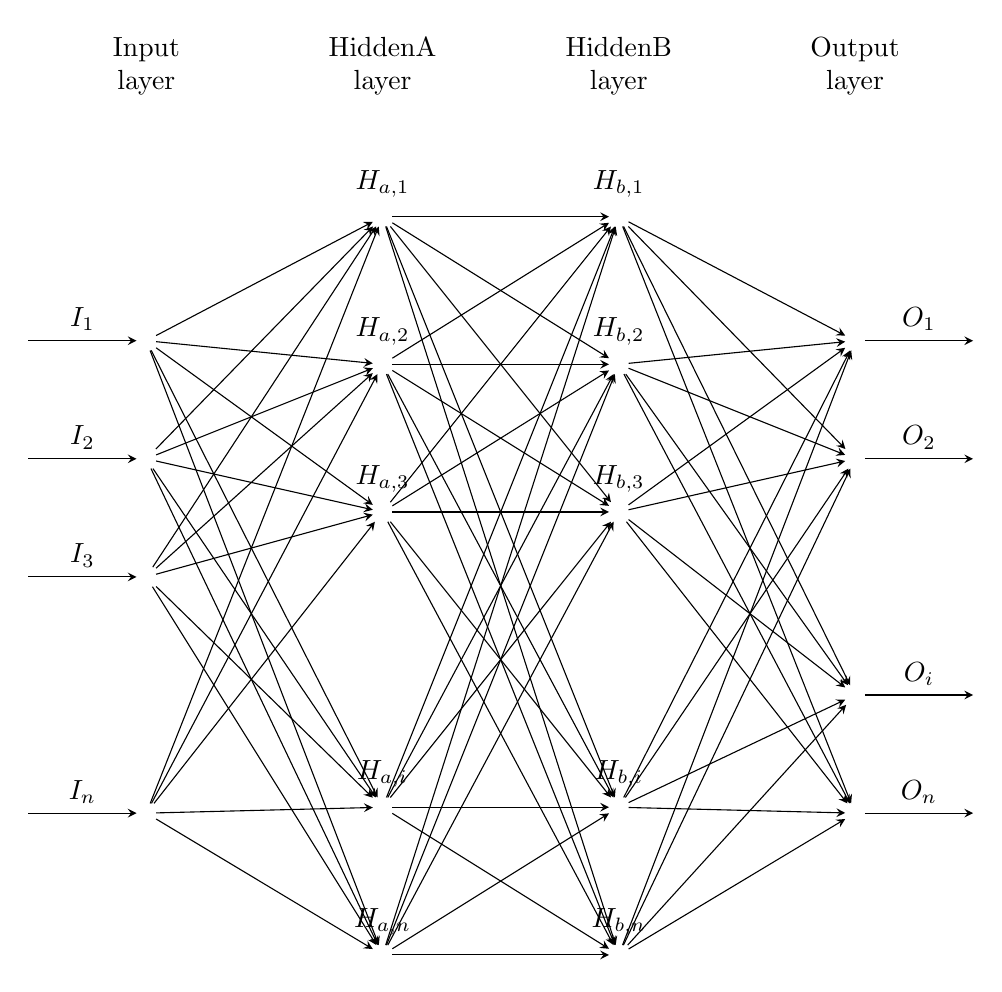
\begin{tikzpicture}[x=1.5cm, y=1.5cm, >=stealth]

    \foreach \m/\l [count=\y] in {1,2,3,missing,4}
      \node [every neuron/.try, neuron \m/.try] (input-\m) at (0,1-\y) {};
    
    \foreach \m [count=\y] in {1,2,3,missing,4,5}
      \node [every neuron/.try, neuron \m/.try ] (hiddenA-\m) at (2,2.3-\y*1.25) {};
    
    \foreach \m [count=\y] in {1,2,3,missing,4,5}
      \node [every neuron/.try, neuron \m/.try ] (hiddenB-\m) at (4,2.3-\y*1.25) {};
      
    \foreach \m [count=\y] in {1,2,missing,3,4}
      \node [every neuron/.try, neuron \m/.try ] (output-\m) at (6,1-\y) {};
    
    \foreach \l [count=\i] in {1,2,3,n}
      \draw [<-] (input-\i) -- ++(-1,0)
        node [above, midway] {$I_\l$};
    
    \foreach \l [count=\i] in {1,2,3,i,n}
      \node [above] at (hiddenA-\i.north) {$H_{a,\l}$};
    
    \foreach \l [count=\i] in {1,2,3,i,n}
      \node [above] at (hiddenB-\i.north) {$H_{b,\l}$};
    
    \foreach \l [count=\i] in {1,2,i,n}
      \draw [->] (output-\i) -- ++(1,0)
        node [above, midway] {$O_\l$};
    
    \foreach \i in {1,...,4}
      \foreach \j in {1,...,5}
        \draw [->] (input-\i) -- (hiddenA-\j);
    
    \foreach \i in {1,...,5}
        \foreach \j in {1,...,5}
            \draw [->] (hiddenA-\i) -- (hiddenB-\j);  

    \foreach \i in {1,...,5}
      \foreach \j in {1,...,4}
        \draw [->] (hiddenB-\i) -- (output-\j);
    
    \foreach \l [count=\x from 0] in {Input, HiddenA, HiddenB,Output}
      \node [align=center, above] at (\x*2,2) {\l \\ layer};
    
    \end{tikzpicture}
\end{center}
A network can be represented as a function $f$ parameterised by weight
matrix $\mathbf{W}$ and bias matrix $\mathbf{b}$ with the outputs of each
layer being passed into the next layer in a fully connected network.
\begin{equation}
    \mathbf{\hat{y}}= f(\mathbf{x}; \mathbf{W}, \mathbf{b})
\end{equation}
The network is optimised against a target output $Y$ using stochastic gradient descent.
\begin{equation}
    \begin{gathered}
        L(Y, \mathbf{\hat{y}}) = \Vert Y - \mathbf{\hat{y}} \Vert_{2} \\
        = \frac{1}{N} \cdot \sum_{i=1}^{N} (Y_i - (\mathbf{x}_i \cdot \mathbf{w}_i^\top + b))^2
    \end{gathered}
\end{equation}
\begin{equation}
    \begin{gathered}
        \frac{\partial E}{\partial \mathbf{w}} = -\frac{2}{N} \cdot \sum_{i=1}^{N} \mathbf{x}_i(Y_i-(\mathbf{x}_i \cdot \mathbf{w}_i^\top +b)) \\
    \frac{\partial E}{\partial b} = -\frac{2}{N} \cdot \sum_{i=1}^{N} (Y_i-(\mathbf{x}_i \cdot \mathbf{w}_i^\top +b))
    \end{gathered}
\end{equation}
\begin{gather}
    \begin{aligned}
        \nabla_{\mathbf{W}} E = \frac{\partial L(Y, \mathbf{\hat{y}}) }{\partial \mathbf{W}}  \,, \;\;\; &
        \nabla_{\mathbf{b}} E = \frac{\partial L(Y, \mathbf{\hat{y}})}{\partial \mathbf{b}} \,
    \end{aligned} 
\end{gather}
The error is calculated first for the network's output layers, the weights are then updated in the direction of 
negative gradient, steepest descent with respect to error $E$ with some constant stepsize $\eta$:
\begin{equation}
    \mathbf{W}_{k+1}=\mathbf{W}_{k} - \eta \nabla E_{\mathbf{W}_k}
\end{equation}
The gradients for the biases are updates likewise. This error is then back-propagated
using reverse mode differentiation on a computational graph \cite{Margossian2019} through the remaining nodes,
where the weights adjusted after the gradient updates are used as the target for the preceeding layer.
\begin{remark}
    In recent years additional properties of neural networks have been discovered
    relating to their nature as universal function approximators. Neural networks with
    a single hidden layer can approximate any function, and as the number
    of nodes tends to infinity it simplifies to a linear model \cite{Jaehoon2019}. Alternatively, infinitely
    wide, deep neural networks are equivalent to a gaussian process \cite{Jaehoon2017}.
    The have also demonstrated the ability to sort lists in practically $O(1)$ time \cite{Xiaoke2019}.
\end{remark}
\subsubsection{Deep Q-Networks}
Neural networks can be used to approximate the Q function directly using Q learning, however the structure
of the gradient update introduces complexity when trying to estimate expected value of rewards. We begin by 
parameterising our Q fuction with the weights of our network:
\begin{equation}
    \begin{gathered}
        Q(s,a)= f(\mathbf{s}; \mathbf{W}, \mathbf{b}) \;\;\;\; s \in \mathbf{S}\\
        \Rightarrow Q(s,a ; \mathbf{W}, \mathbf{b}) \rightarrow Q(s,a ; \mathbf{W}) \\
    \end{gathered}
\end{equation}
We can develop a loss function in the off policy setting using the Bellman Error $\delta_t$.
This holds because the update target $R_{t+1} + \gamma \max_a Q(S_{\textcolor{red}{t+1}},a)$ acts as a
"peek ahead" from the perspective of the current state. That is we take an action, observe the
outcome, and update the action-value of our old state with this new information.
\begin{equation}
    \begin{gathered}
        L(\delta_t, Q(s,a; \mathbf{W})) = \Vert \delta_t - Q(s,a; \mathbf{W}) \Vert_2 \\
        \frac{\partial L(\delta_t, Q(s,a;\mathbf{W} )) }{\partial \mathbf{W} } = \frac{\partial (\delta_t - Q(s,a; \mathbf{W}))^2}{\partial \mathbf{W}}\\
        = (\delta_t - Q(s,a; \mathbf{W})) \cdot \frac{\partial (\delta_t - Q(s,a; \mathbf{W}))}{\partial \mathbf{W}} \\
        = (\delta_t - Q(s,a; \mathbf{W})) \nabla_{\mathbf{W}} Q(s,a; \mathbf{W})
    \end{gathered}
\end{equation}
The target acts as a constant because the maximal estimated Q value at the next state is taken
to be the value of the state under the optimal policy (see 2.32). In their original paper, \cite{Mnih2015}
used a neural network to take in the state as input and then output a vector of action values, 
one for each action. If we used the intepretation of Q learning developed in (2.41), this structure could lead to unstable
gradient updates or could cause the action values to diverge. This can be described
in terms of the correlation between various elements of the model, consider
two dependent random variables $X$ and $Y$:
\begin{equation}
    \begin{gathered}
        Correlation(X,Y) = \frac{Covar(X,Y)}{\sqrt{Var(X)Var(Y)}} \\
        %Correlation(X,Y) \propto Covar(X,Y) \\
        %Correlation(X,Y) \propto \mathbb{E}[(X - \mathbb{E}[X])(Y - \mathbb{E}[Y])] \\
        %\propto \mathbb{E}[XY - X\mathbb{E}[Y] - Y\mathbb{E}[X] + \mathbb{E}[X]\mathbb{E}[Y]] \\
        %\propto \mathbb{E}[XY] - \mathbb{E}[X]\mathbb{E}[Y] - \mathbb{E}[Y]\mathbb{E}[X] + \mathbb{E}[X]\mathbb{E}[Y] \\
        %\propto \mathbb{E}[XY] - \mathbb{E}[X]\mathbb{E}[Y]\\
    \end{gathered}
\end{equation}
The corelation between two dependent random variables is proportional to the covariance of
the random variables normalised by their joint standard deviatiation $\sqrt{Var(X)}= \sigma$.
As correlation is a dimensionless constant on the interval $[-1,1]$, if $X$ and $Y$ are
correlated $Corr(X,Y) \approx 1$, then they increasingly co-vary across each dimension, then their
standard deviation must increase likewise, and as the co-variance goes to infinity, so does their
individual variance. And so under (2.41) we would be using a very similar distribution of
weights to calculate $\max_a Q(S_{t+1}, a)$ and $Q(S_{t}, a)$ which are both dependent 
according to the definition of our MDP. In addition to that, if we consider
successive frames of pixels on a screen as our states, it is trivial note that these
observations will also be highly correlated; in the case of the atari game "Pong", the
position on the paddle on the next frame is highly informed by position of the paddle in the next frame.

Instead, \cite{Mnih2015} propose two solutions to this problem. A biologically
inspired mechanism termed \emph{Experience Replay} and a separate \emph{Target Network}.
To remove the correlations between succesive observations $(S_t,A_t,R_{t+1},S_{t+1})$, they
instead store these tuples in a \emph{replay buffer}. In this case the replay buffer is a FIFO
array of constant size that overwrites older memories with new ones. The target network
is a seperate neural network whose weights $\theta^-$ are initialised with the weights of
the behaviour network and then frozen. Periodically, this target network is updated with the
current weights of the behaviour network $\theta$. 
Every timestep, a batch of memories are uniformly sampled, the target network is used to compute the Bellman Error
for each memory and the output of the behaviour network is updated according to the loss defined in (2.49),
averaged across the whole batch.
This algorithm proceeded to lead a breakthrough in contemporary deep reinforcment learning by outperforming
human benchmarks at a super human level for the first time (adapted from the original authors):
\begin{algorithm}[!htb]
    \SetAlgoLined
    \caption{Deep Q Network (DQN)}
    Init replay memory $D$ to capacity $N$ \;
    Init $Q$ with random weights $\theta$\;
    Init $\hat{Q}$ with $\theta^- = \theta$\;
    \ForAll{episodes}{
        Init state $s_1$\;
        Preprocess sequence $\phi_1 = \phi(s_1)$\;
        \ForAll{timesteps in episode}{
            $r \backsim U(0,1)$\;
            \eIf{r < $\varepsilon$}{
                $a_t \backsim {A}$ \tcp*[l]{ Randomly sample action from action space}
            }{
                $a_t = \underset{a}{argmax}\;\;Q(\phi(s_t),a ; \theta)$\;
            }
            Execute action $a_t$ observe $R_{t+1}, s_{t+1}, d$ \tcp*[l]{$d = 1$ if state is terminal else $0$} 
            Store $(\phi_1,a_t,r_{t+1},\phi_{t+1})$ in $D$\;
            Sampled random minibacth from $D$\;
            $\delta_t = r_t + (1-d) \gamma \max_{a'} \hat{Q}(\phi_{t+1},a'; \theta^-)$\;
            Perform gradient update $(\delta_t - Q(s,a; \theta)) \nabla_{\theta} Q(s,a; \theta)$\;
            Every $C$ steps reset $\hat{Q} = Q$\;
        }
    }
\end{algorithm}

\subsection{Improvements to Vanilla Deep Q-Networks}
The success of the original DQN algorithm was not without flaws however.
\subsubsection{Memory}
\subsubsection{Exploration}
\subsubsection{Exploitation}
\subsubsection{Rainbow DQN}